\section{РАЗРАБОТКА ВЕБ-ПРИЛОЖЕНИЯ}

\subsection{Реализация подсистемы аутентификации и проверки ролей}

Основой безопасности разрабатываемого приложения является подсистема аутентификации, реализованная с помощью библиотеки \texttt{Flask-Login}. Хранение паролей в базе данных осуществляется в зашифрованном виде с использованием криптографических хэш-функций из модуля \texttt{werkzeug.security} \cite{werkzeug_doc} (функции \texttt{generate\_password\_hash} и \texttt{check\_password\_hash}).

Для разграничения прав доступа была внедрена ролевая модель (RBAC). При выполнении критически важных действий на стороне сервера происходит проверка атрибута \texttt{role} текущего пользователя.

Листинг 1 --- Фрагмент кода проверки прав доступа при создании проекта
\begin{Verbatim}[frame=single, numbers=left, fontsize=\small, xleftmargin=5mm, tabsize=4]
@app.route('/create_project', methods=['POST'])
@login_required
def create_project():
    if current_user.role != 'admin':
        flash('У вас нет прав для создания проектов.', 'danger')
        return redirect(url_for('index'))
        
    title = request.form.get('title')
    description = request.form.get('description')
    
    if title:
        new_project = Project(title=title, description=description, 
                              owner_id=current_user.id)
        db.session.add(new_project)
        db.session.commit()
    return redirect(url_for('index'))
\end{Verbatim}

На рисунках \ref{fig:screen_register} и \ref{fig:screen_login} представлены интерфейсы страниц регистрации и входа в систему.

\begin{figure}[h!]
    \centering
    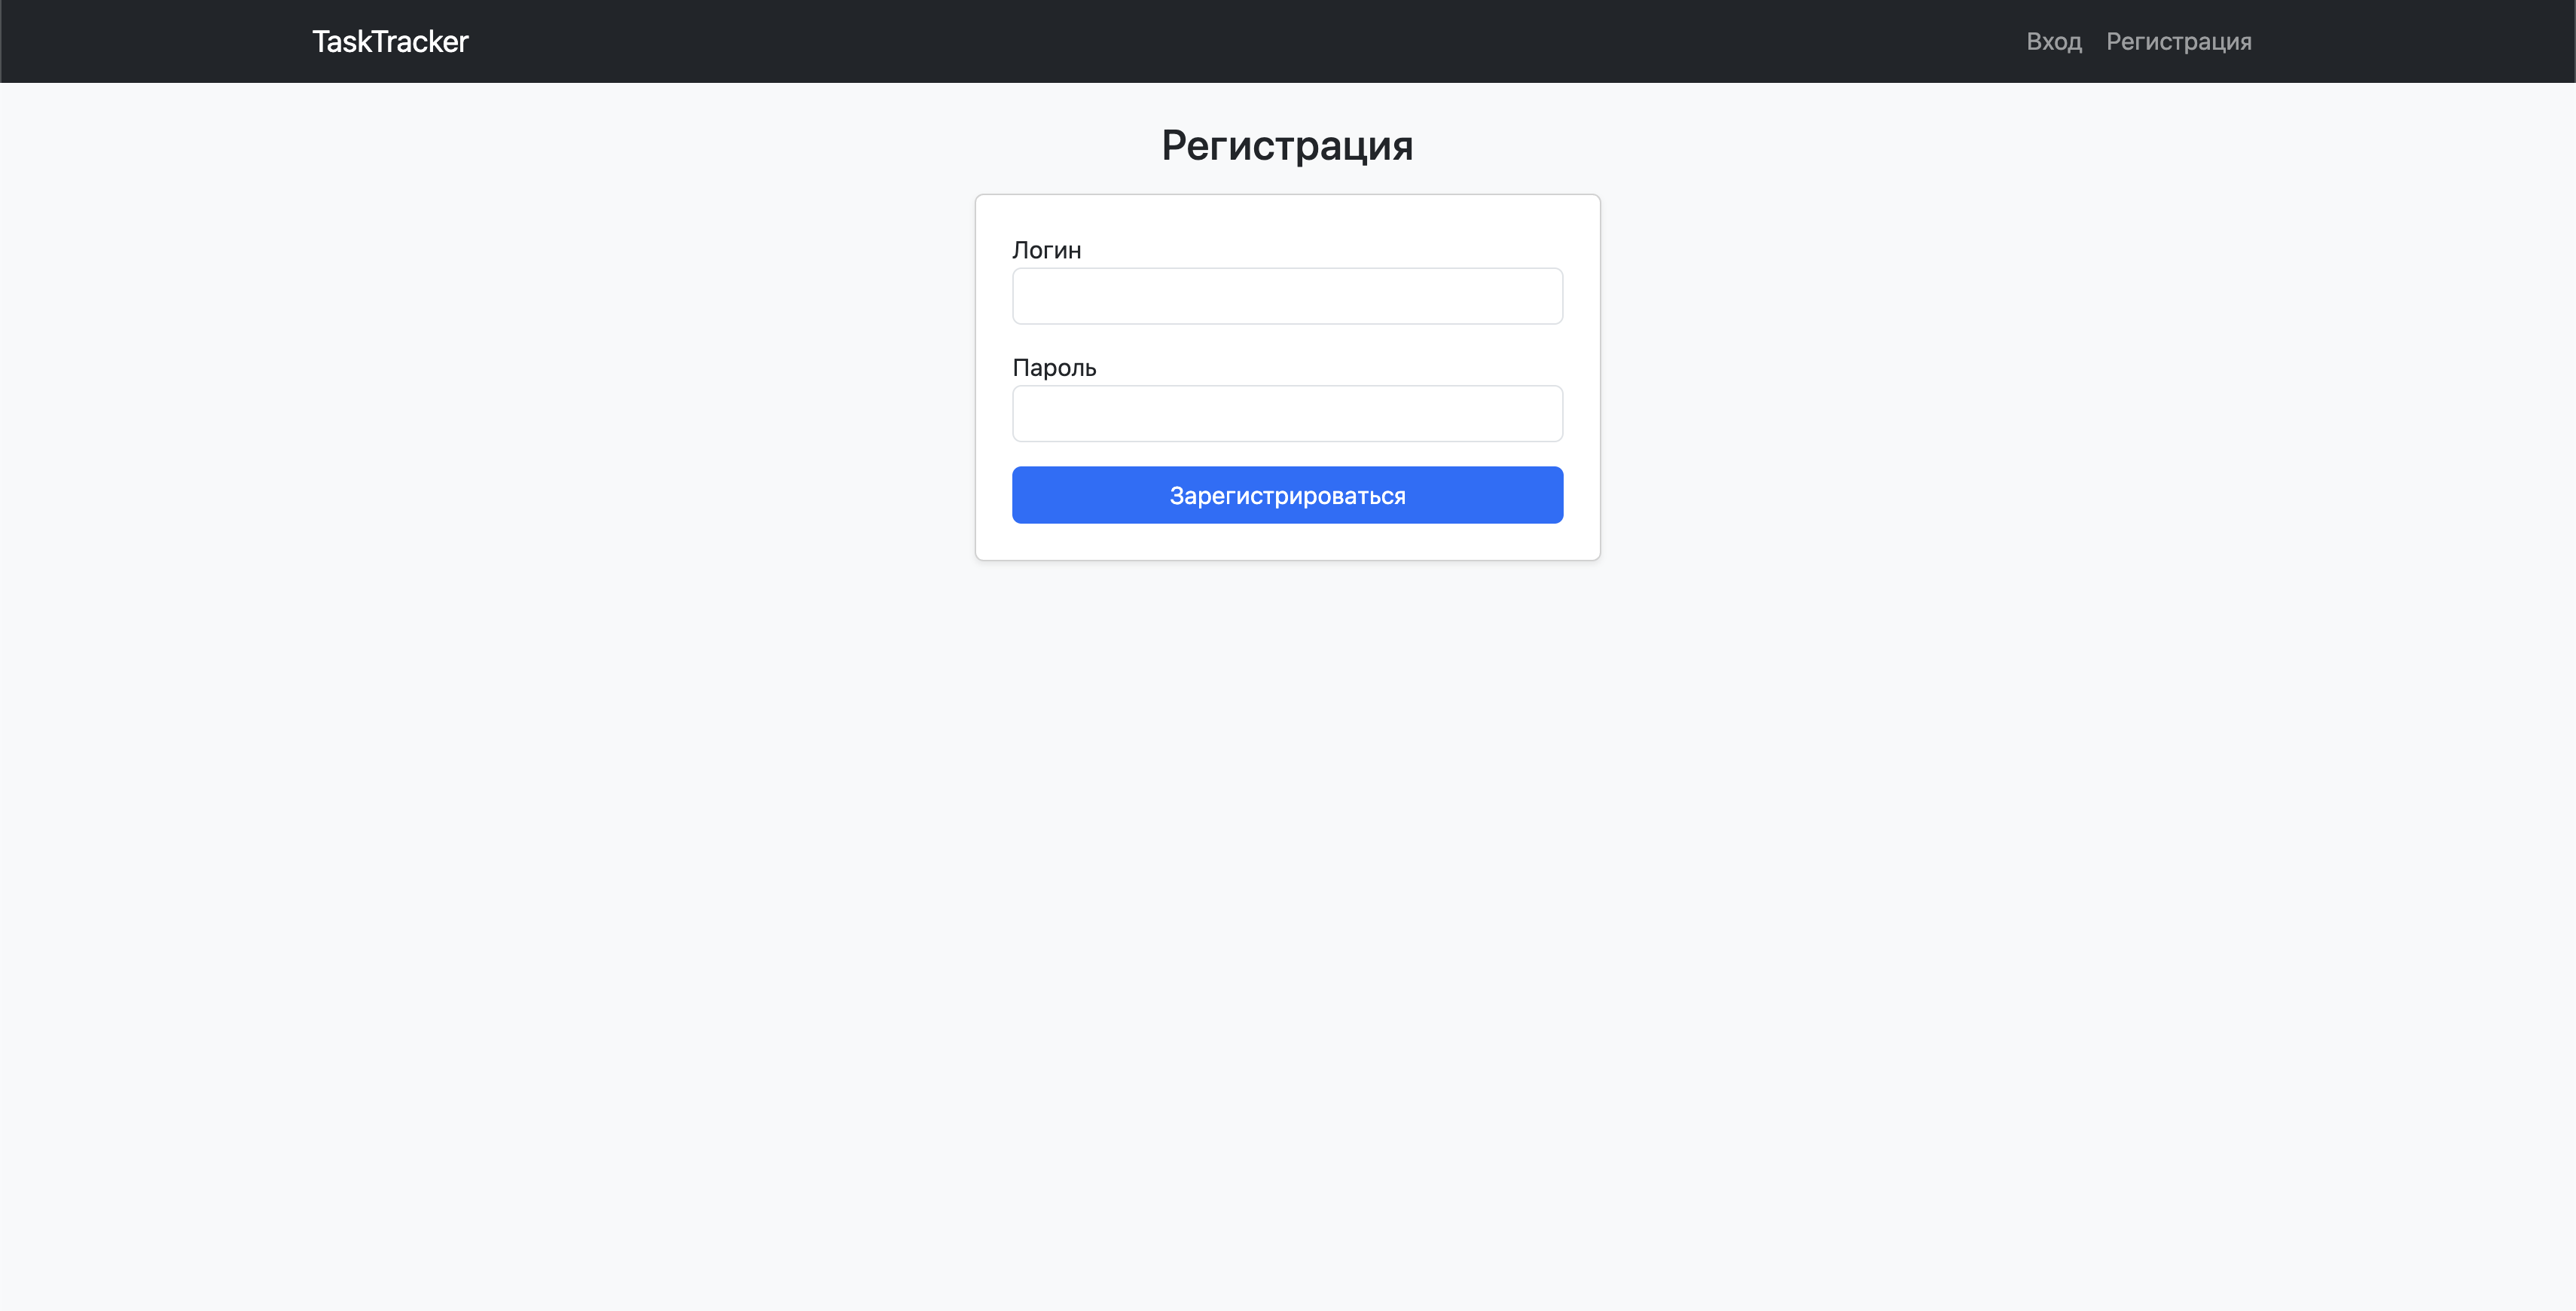
\includegraphics[width=0.8\textwidth]{images/screen_register.png}
    \caption{Страница регистрации}
    \label{fig:screen_register}

    \vspace{1cm}

    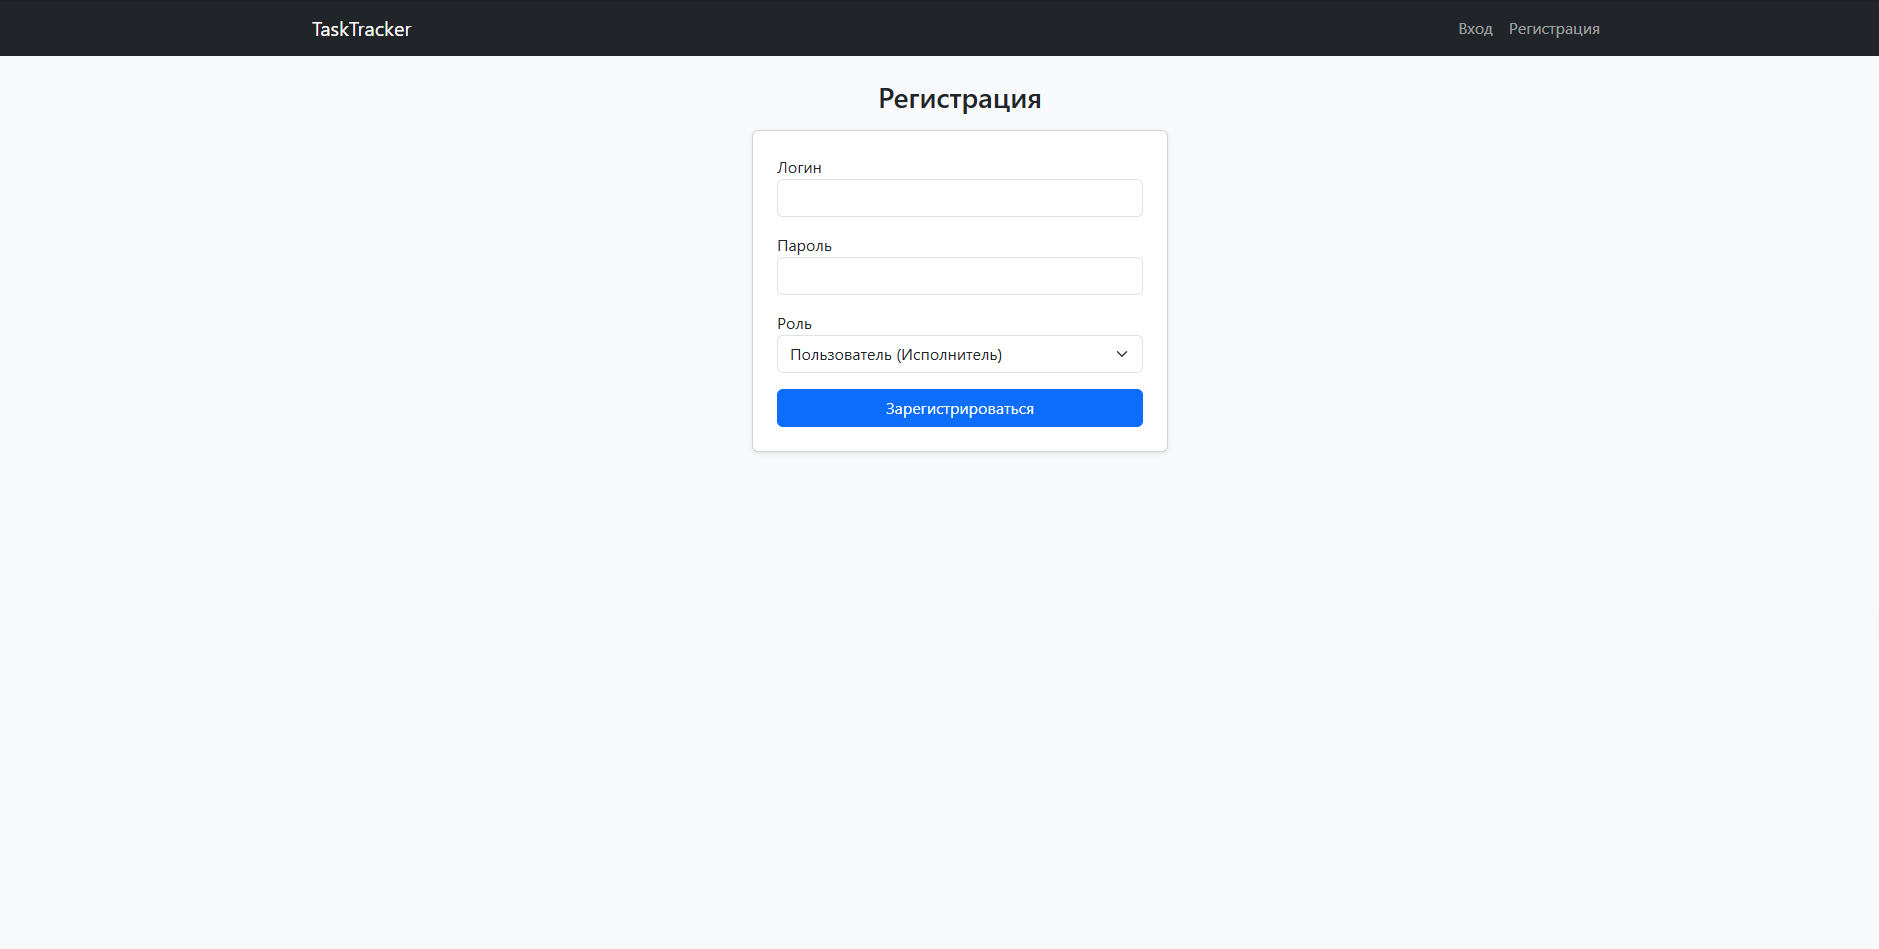
\includegraphics[width=0.8\textwidth]{images/screen_login.png}
    \caption{Страница авторизации}
    \label{fig:screen_login}
\end{figure}

\clearpage 

\subsection{Разработка CRUD-интерфейсов и работы с файлами}

Управление сущностями системы осуществляется через реализованные CRUD-интерфейсы. Взаимодействие с реляционной базой данных PostgreSQL инкапсулировано через объектно-реляционное отображение \texttt{SQLAlchemy}. 

Особое внимание уделено безопасной работе с файлами и возможности множественного прикрепления документов к одной задаче. Для защиты файловой системы сервера используется утилита \texttt{secure\_filename}, а для предотвращения коллизий реализована генерация уникальных префиксов на базе библиотеки \texttt{uuid}. Кроме того, внедрен механизм автоматического физического удаления файлов с жесткого диска при удалении проекта или задачи.

На рисунке \ref{fig:screen_project} продемонстрирован интерфейс управления задачами конкретного проекта, включающий таблицу задач, элементы фильтрации и навигации.

\begin{figure}[h!]
    \centering
    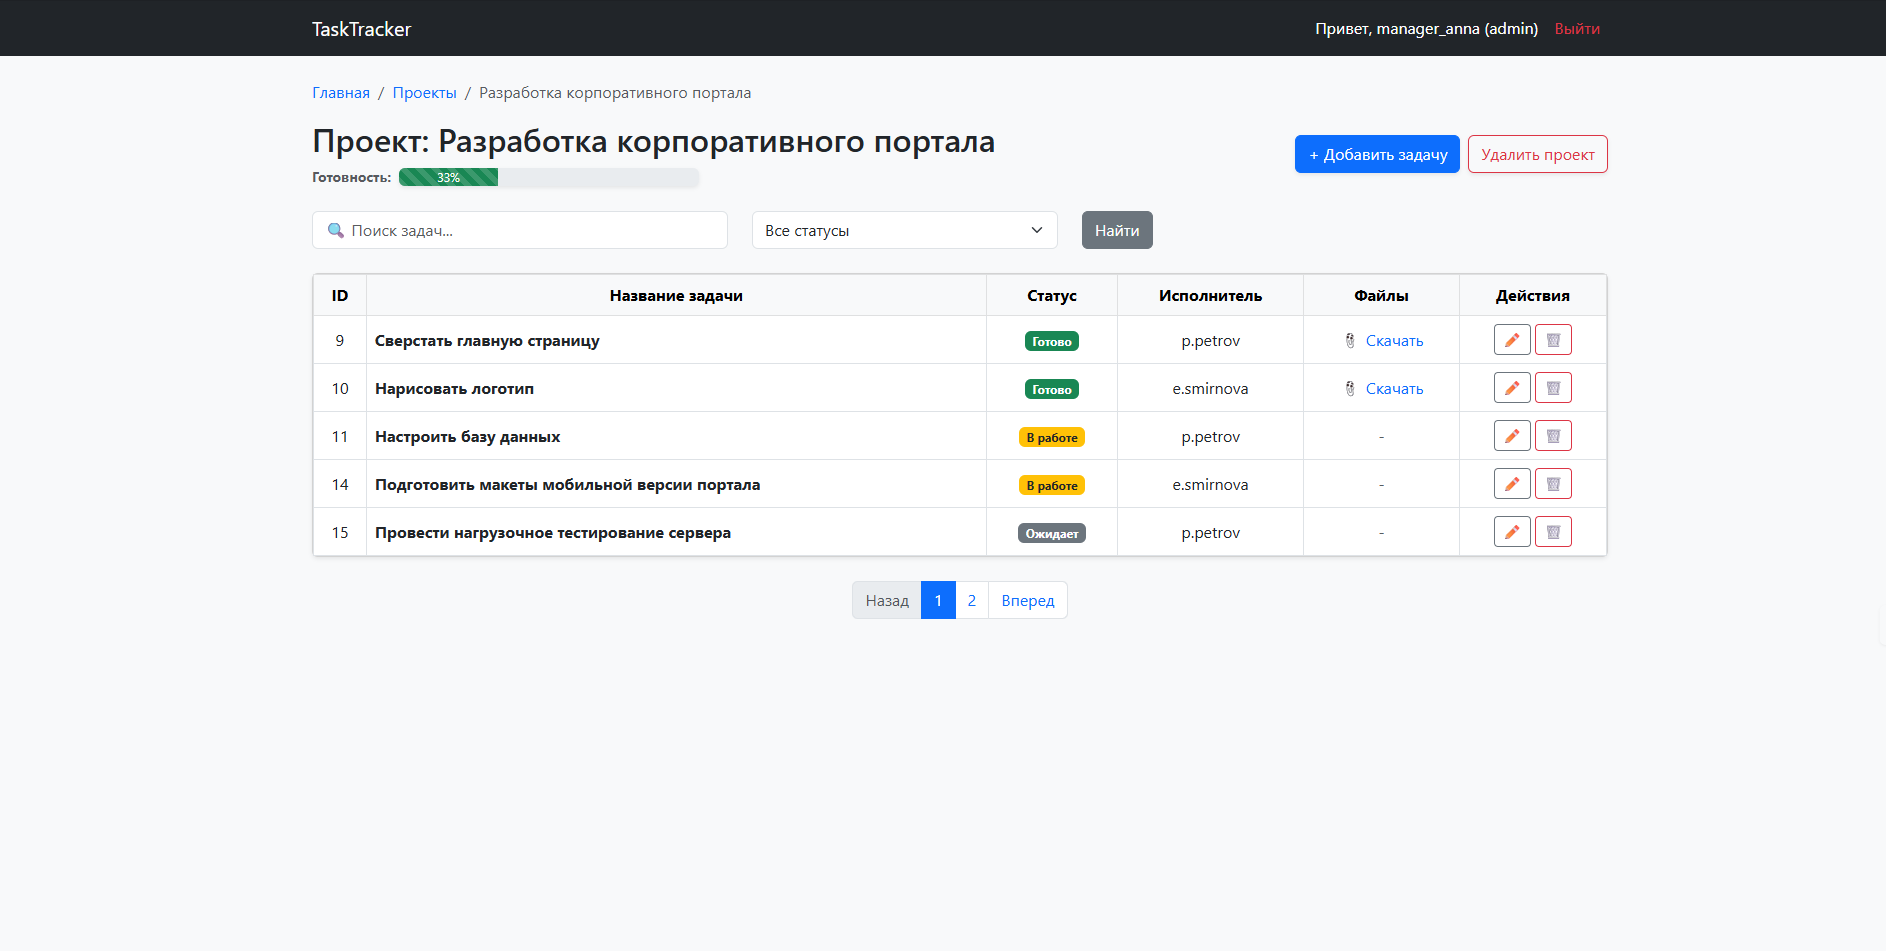
\includegraphics[width=0.85\textwidth]{images/screen_project.png}
    \caption{Интерфейс управления задачами проекта}
    \label{fig:screen_project}
\end{figure}

\clearpage

\subsection{Реализация модуля агрегирования данных}

Для обеспечения администратора системы наглядной аналитикой был разработан модуль агрегирования данных. На серверной стороне с помощью агрегатных функций SQLAlchemy (метод \texttt{.count()}) выполняется подсчет задач, сгруппированных по их текущему статусу. 

Полученные статистические данные передаются в HTML-шаблоны, где визуализируются в двух форматах: в виде динамической шкалы готовности (Progress Bar) внутри каждого проекта и в виде интерактивной круговой диаграммы на базе библиотеки \texttt{Chart.js} \cite{chartjs_doc} на главной панели управления. Результат работы модуля представлен на рисунке \ref{fig:screen_dashboard}.

\begin{figure}[h!]
    \centering
    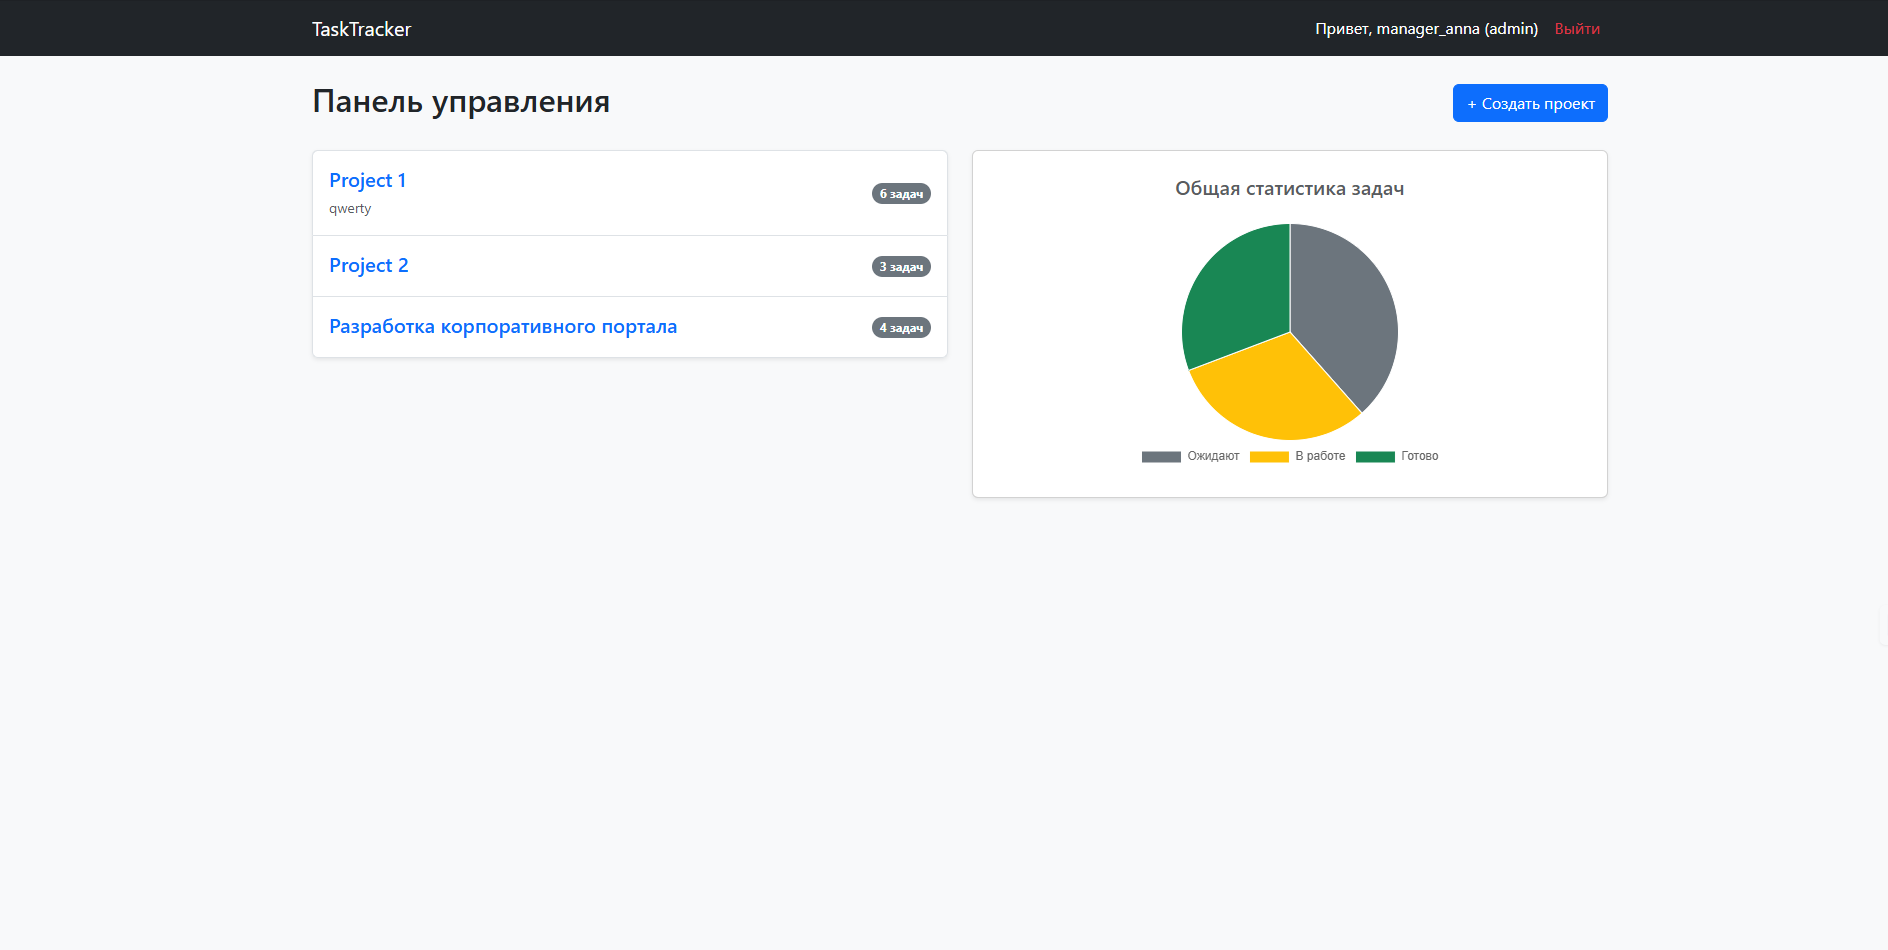
\includegraphics[width=0.85\textwidth]{images/screen_dashboard.png}
    \caption{Главная панель управления (Дашборд) с круговой диаграммой}
    \label{fig:screen_dashboard}
\end{figure}

Листинг 2 --- Фрагмент кода агрегации данных в базе
\begin{Verbatim}[frame=single, numbers=left, fontsize=\small, xleftmargin=5mm, tabsize=4]
# Агрегирование данных для круговой диаграммы
total_tasks = Task.query.count()
pending_tasks = Task.query.filter_by(status='pending').count()
in_progress_tasks = Task.query.filter_by(status='in_progress').count()
done_tasks = Task.query.filter_by(status='done').count()

stats = {
    'total': total_tasks,
    'pending': pending_tasks,
    'in_progress': in_progress_tasks,
    'done': done_tasks
}
\end{Verbatim}